%-----------------------------------------------------------------------
% Latex Thesis/Dissertation Template for Wright State University
% 
% Written by Sean A. Mortara
% 28 June 2001
% Modified by Josh Mark
% 15 Dec 2011
% Later edits by Joseph C. Slater
%-----------------------------------------------------------------------
\documentclass[12pt]{report}

\usepackage{xcolor}
\usepackage{booktabs} % used for tables
\usepackage{multirow} % used for tables to merge multiple rows
\usepackage{bigdelim} % used for tables to set spacing
\usepackage{bigstrut} % used for tables to set spacing
\usepackage{graphicx} % used for includegraphics
\usepackage{subfigure} % allows the use of subfigures
\usepackage[framed,numbered,autolinebreaks,useliterate]{mcode} % used to insert code
%
%
%



%-----------------------------------------------------------------------
%  Modified fields
%-----------------------------------------------------------------------
\newcommand{\authorfirst}{Johnny}
\newcommand{\authorMI}{B.~}
\newcommand{\authorlast}{Goode}
\newcommand{\degreefull}{Mas\-ter of Sci\-ence in En\-gi\-neer\-ing}  % force hyphenation at syllables if line breaks are required
\newcommand{\degreeshort}{M.S.Egr.}
\newcommand{\thesisordissertationlc}{dissertation}
\newcommand{\dept}{Department of Lollipops}
\newcommand{\institution}{Wright State University} % Doubting you will
                                % change this. 
\newcommand{\thesistitle}{Some Really Great Title That Provides a
  Con\-cise View of the Topic Your Thesis Will Address} % Needes a line break
\newcommand{\bachdegreeshort}{B.S.M.E.} % Bachelor degree short
\newcommand{\bachinstitution}{Universal University} % Bachelor degree institution
\newcommand{\bachyear}{2004}% Bachelor degree year
%No spaces should be before or after this title.
\newcommand{\pdfsubject}{a short paraphrase of your title or focus of your thesis}
\newcommand{\pdfkeywords}{keyword 1, keyword 2, keyword 3, keyword 4}
\newcommand{\yearcomplete}{2013}
% set pdf file info
\usepackage{hyperxmp} % used to set pdf property info with \hypersetup command

%-----------------------------------------------------------------------
%  Thesis Advisor, Department Chair, Dean of Graduate Studies
%  I don't know why titles as separated... except in the one case at
%  the end. 
%-----------------------------------------------------------------------
\newcommand{\thesisdirector}{Advisor's Name}
\newcommand{\thesisdirectortitle}{Ph.D., P.E.}
\newcommand{\deptchair}{Al Yankovic}
\newcommand{\deptchairtitle}{Ph.D., P.E.}
\newcommand{\dean}{Elmer Fudd, PhD, MD, FEP}
\newcommand{\deantitle}{Vice President for Research and\\ Dean of the
  Graduate School}
%-----------------------------------------------------------------------
%  Final Examination Committee: Comment out the ones you don't need. 
%-----------------------------------------------------------------------
\newcommand{\fecone}{Committee member 1}

\newcommand{\fectwo}{Committee member 2}

\newcommand{\fecthree}{Committee member 3}

\newcommand{\fecfour}{Committee member 4}

\newcommand{\fecfive}{Committee member 5}

\newcommand{\fecsix}{Committee member 6}

\newcommand{\fecseven}{Committee member 7}

% If you have more committee members... good luck

% Modify this if needed for getting citations to "look right" according to your field. Read the natbib documentation on how to use this. 
%\usepackage[round]{natbib}
%\usepackage{doublespace}

%=============================
%  Begin document!
%=============================
%
% Don't touch

% still don't touch.   

% title sheet
\usepackage{WSU}
\hypersetup{
                     pdfauthor={\authorfull},
                     pdftitle={\thesistitle},
                     pdfsubject={\pdfsubject},
                     pdfkeywords={\pdfkeywords},
                     }
% \normalem
\pagenumbering{roman}
\pagestyle{plain}
\rhead{\today}
\begin{document}
\maketitle
\doublespace

% Still don't touch!!

%=============================
%  approval sheet
%=============================

\thispagestyle{empty}
\renewcommand\baselinestretch{2}
\begin{singlespace}
\signaturepage
\end{singlespace}
%
%=============================
%  Abstract
%=============================
\newpage
\setcounter{page}{3}
\vspace{2in}
%
\begin{singlespace}
\begin{center}
  ABSTRACT
\end{center}
%
\noindent{\small{\authorlast, \authorfirst}. 
		 {\degreeshort, \dept, \institution}, 
		 {\yearcomplete}. 
		 {\sl \thesistitle}.}
\end{singlespace}
\vspace*{.5in}

\pdfbookmark[0]{Abstract}{Abstract}
%\phantomsection
%
%========================
% Start editing below. 
%========================
The abstract should succinctly summarize the contents of the thesis, stating the problem, the procedure or methods used, the results, and any conclusions.  Doctoral dissertation abstracts should not exceed 350 words.  Master's thesis abstracts should not exceed 150 words.
%%%%%%%%%%%%%%%%%%
%-----------------------------------------------------------------------
%
%=============================
%  List of symbols (Optional)
%=============================
\newpage
%\renewcommand\baselinestretch{1.5}
\begin{singlespace}\begin{center}
  \textbf{\Huge{List of Symbols}}
\end{center}

\begin{flushleft}{\large Chapter 2} \end{flushleft}
\begin{tabular}{p{0.75in}l}
   $\gamma$ & $\frac{-b+\sqrt{b^{2}-4ac}}{2a}$\\
   $L$ & {Plate length}\\
\end{tabular}

%%%%%
\begin{flushleft}{\large Chapter 3} \end{flushleft}
\begin{tabular}{p{0.75in}l}
   $h$ & {Plate thickness}\\
   $L$ & {Plate length}\\
\end{tabular}

%%%%%
\begin{flushleft}{\large Chapter 4} \end{flushleft}
\begin{tabular}{p{0.75in}l}
   $M_{\infty}$ & {Freestream Mach number}\\
   $U_{\infty}$ & {Freestream fluid velocity}\\
   $p-p_\infty$ & {Aerodynamic pressure differential}\\
\end{tabular}

%%%%%
\begin{flushleft} {\large Chapter 7} \end{flushleft}
\begin{tabular}{p{0.75in}l}
   $\beta$   & $\sqrt{M_{\infty}^2-1}$\\
   $\lambda$ & {Nondimensional freestream dynamic pressure}\\
\end{tabular}
\end{singlespace}

%=============================
%  Table of contents, etc.
%=============================
%\renewcommand\baselinestretch{1.5}
\begin{singlespace}
\tableofcontents
\listoffigures
\listoftables
\end{singlespace}
%
%=============================
%  Acknowledgments
%=============================
\newpage
\thispagestyle{plain}
\setlength{\parindent}{0em}
\begin{center}
{\huge Acknowledgment}
\end{center}

I would like to take this opportunity to extend my thanks to\ldots If you have multiple paragraphs, the first should not be indented to match the style of the rest of the thesis

\setlength{\parindent}{2em}
Any additional paragraphs should be indented as such.  Remember to thank your advisor and committee members.
%
%=============================
%  Dedication
%=============================
\newpage
\thispagestyle{plain}
\vspace*{3in}
\begin{center}
Dedicated to\\
Somebody special (Wife, husband, girlfriend or boyfriend works well
here. )
\end{center}
%
%
%
%=============================
%  Begin Chapters
%=============================
\newpage
\setcounter{page}{1}
\pagenumbering{arabic}
\setlength{\parindent}{2em}
%=============================
\chapter{In The Beginning}
%=============================
The date of this document generation (current version of this document) is the date of the thesis on page two (\today).{}
sdafsd sadfsdaf asdfadf. OK, I have nothing to say here, but you should in your thesis/dissertation. Introduce your chapter in a page or so. 

On a side note, style files should be located in the texmf tree automatically when a package is installed.  The sty-files used for this template are located in the folder \lq\lq{}sty\_files\_if\_needed\rq\rq{}.  If you do not have the packages already installed, you can also simply move or copy them into the same directory as this file.

%=============================
\section[Citations/References (short form of section name)]{Citations, using them, referring to them, formatting them, and loving using them because if you don't use them when appropriate it's called \emph{plagiarism}, and references}
%=============================
That was a ridiculously long section name to illustrate how to get a shorter version in your table of contents.  

See section \ref{sec:equations}. I'm not the only one who says this is awesome stuff\cite{Mortara2004}!
This citation is in the ASME format (for which I've included a bst file. See \textsc{asmems4} in the source document(way near the end). Some  other options are:
\begin{itemize}
\item natbib:  put \verb'\usepackage{natbib}' in the header (before \verb'\begin{document}'), and \verb'\bibliographystyle{plainnat}' just before \verb'\bibliography').  See the natbib documentation for details.
\item AIAA:  put \verb'\usepackage{overcite}' in the header (before \verb'\begin{document}'), and \verb'\bibliographystyle{aiaa}' just before \verb'\bibliography'). Use \verb'\citen{sdfsdf}' for in-line citations. Read the overcite package documentation for more. 
\end{itemize}

A variety of other formats are available on \href{http://www.ctan.org}{CTAN} or though an internet search. You may also just pick one using ''natbib''.\footnote{Don't those quotes look bad before ``natbib''? Well, use two left quotes in \LaTeX\ to get it to look right.}  The formatting of your references is controlled by the \verb'bibliographystyle' command near the end of the document. Use the bibliography style appropriate to your field. On exists, out there. I'm sure. If not (ok, it happened to me 10 years ago), you can use the \verb'makebst' script to make your own. Answer a bunch of questions and it makes a style file for you. If you are using a numerical citation system, you may want to use \verb'\usepackage{cite}'. It creates a condensed numerical list of citations, but can cause conflicts with the \verb'hyperref' package (you may need to decide\ldots sorry, this is a bug that drives me nuts too.)

%=============================
\subsection{About the Bibliography}
%=============================
There are two lines in this section in your \LaTeX\ file. The first is a bibligraphystyle command (see the \textsf{tex} file. Don't move it elsewhere. It won't work out well for you.

You need to choose a style file that formats references the way you want them formatted.  You should chose a style for your major.  Look for bst styles on ctan, or use makebst.sty. This formats the bibliography.
The last line is the bibliography command. It just tells \LaTeX\  the name of your \textsf{.bib} file. This is a database of your references. 

Also, use the \verb'\phantomsection' command to correctly anchor the hyperlink for the bibliography.  Without this, any hyperlinks in the document, and the link from the bookmarks will take you to the incorrect page.

You can have as many sources listed in the *.bib file, but if you do not cite them in your document, they will not show up in your Bibliography.  And if you do, they automatically are sorted\ldots pretty nice!  

%=============================
\subsection{Equations}\label{sec:equations}
%=============================
\begin{equation}\label{eq:alphaoverbeta} %You can name the label anything you want, just not the same as something else
x=\frac{\alpha}{\beta}
\end{equation}
Really bad idea: don't start a section with an equation. Don't start a sentence with a variable either. Start with a word. In the body of the text, use the \$ around the variable.  For example, the variable $x$ is the distance. How hard was that?

Sometimes you don't want an equation  number, so use \verb'{equation*}' instead.
\begin{equation*}
x=\frac{-b\pm\sqrt{b^2-4ac}}{2a}
\end{equation*}

If you need to align a set of equations up use the \verb'align' command instead with the use of the \& to set the anchor
\begin{align}
x&=\frac{-b\pm\sqrt{b^2-4ac}}{2a}\\
x&=\frac{\alpha}{\beta}
\end{align}
The same applies for the \verb'align' command\ldots if you don\rq{}t want equation numbers,  just use an *.  More can be found at the references listed in Section \ref{sec:refs}.  You can easily make matrices such as the viscous damping matrix, $C_d$, which is shown in Equation \eqref{eq:damping_mat}.  Use the \verb'\eqref{eq:\ldots}' command to reference equations properly.
%
\begin{equation}
\label{eq:damping_mat}
C_{da} =[U_n^T]^{-1}
\left[ \begin{array}{ccc}
a&b&c\\
	\ddots & 				& \\
	     	& 2 \zeta_i \omega_i 		& \\
		&				& \ddots \\
\end{array} \right]^{{-1}} [U_n]^{-1}
\end{equation}

We don't number equations in \LaTeX. \LaTeX\ does it for us. Label them with names (see the raw \LaTeX\ file).   Just don't put a space in the middle of a variable name. 

Now if I have an equation that I want to be between paragraphs, unlike equation (\ref{eq:alphaoverbeta}), I put a blank line after the equation.
\begin{equation}
  \label{eq:anothersillyequation}
  x\neq y
\end{equation}

See  indent? But if I'm continuing the paragraph, don't put that blank line in
\begin{equation}
  \label{eq:anothersillyequation2}
  x\neq y
\end{equation}
and there won\rq{}t be an indent.

If you want a new page and you have a figure you want to stay with the section, you need to use the \verb'\clearpage' command instead of the \verb'\newpage' command.  

%=============================
\section{Figures}
%=============================
This is not the same as section \ref{sec:equations} on equations. However, if I move that section, I'll still be referring to the right section. 
 Better explained by Figure\footnote{a) Don't use footnotes. b) Capitalize the word ``Figure'')} \ref{fig:example}.  You can keep all of your figures in a sub-directory such as \lq\lq{}pix\rq\rq{}, which is used in this template.
\begin{figure}[htbp] %  figure placement: here, top, bottom, or page
   \centering
   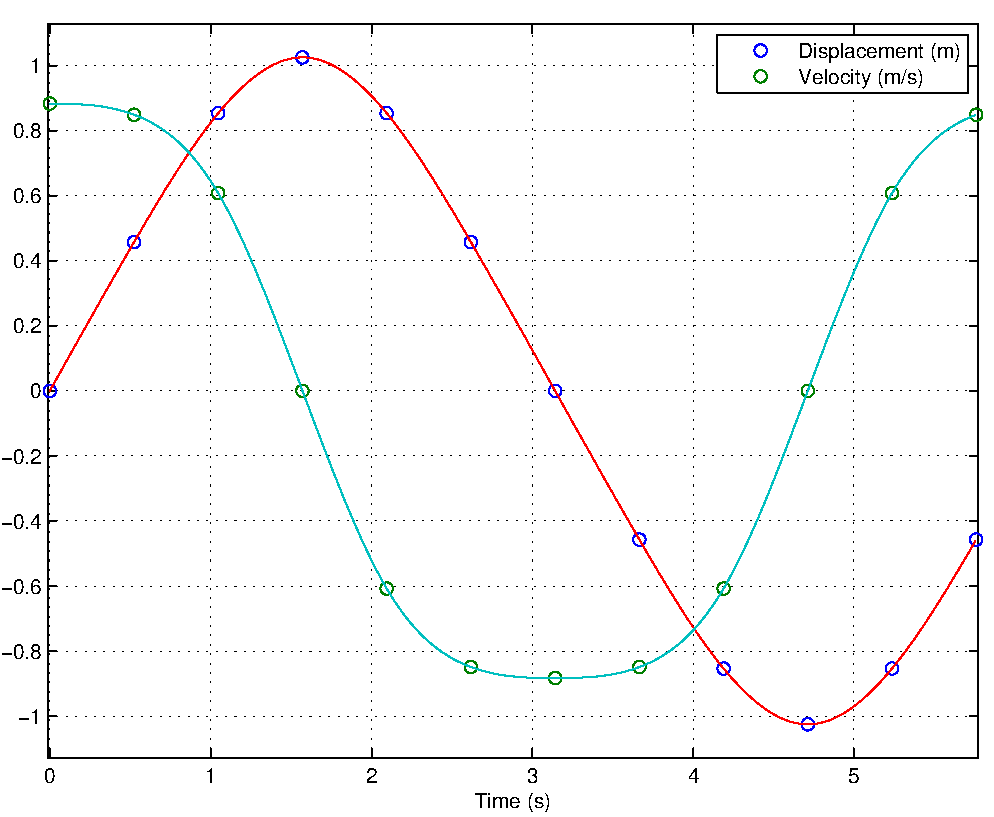
\includegraphics[width=.5\textwidth]{pix/example} %
   \caption{Example caption.}
   \label{fig:example}
\end{figure}

The width of the figure can be set based on percentage of text width as set in Figure \ref{fig:example} or based on inches as used in Figure \ref{fig:example2}.  Also notice the \verb'\label' is after the \verb'\caption'.  This must be true, or the hyperlinks and figure numbers will not be correct.

%----------------------------------------------------------
\begin{figure}[!t] %forced to top of page so no text will be stranded above
   \centering
   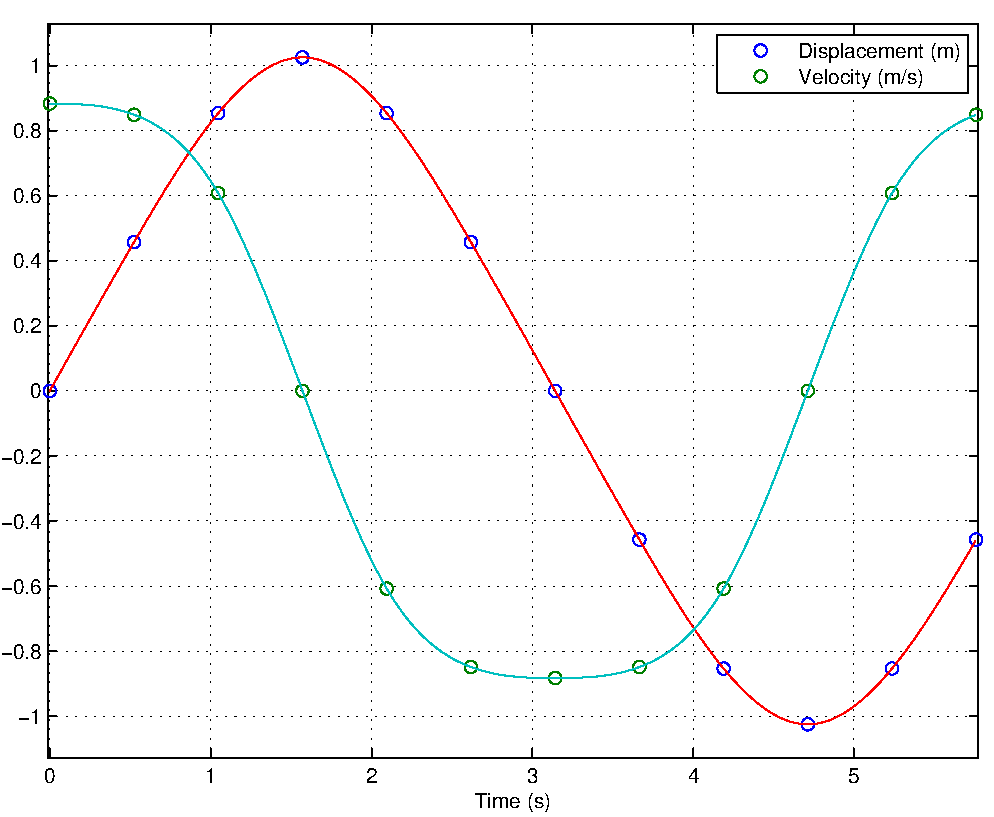
\includegraphics[width=3in]{pix/example} %
   \caption[Short Figure Caption]{Example caption that is way too long for the list of figures, is a run on sentence, has no purpose being this long, except to show you how to avoid such a crazy long entry in your list of figures.}
   \label{fig:example2}
\end{figure}
%----------------------------------------------------------

Don't ask me why the label command has to come late in a figure. It does.  Remember, color won't print well in black and white. Use dashes and dash-dots, etc, for hard copies. I'll document a trick for this later. Basically, make two graphics directories, one for color, one for black and white. Then, use the \textsf{graphicspath} command to choose the one you want. You can Google this for now. 

%=============================
\section{Sub-figures}
%=============================
You can also make sub-figures and reference each of them individually.  You can reference the entire Figure \ref{fig:1x2_subfigs}, or just Figure \ref{fig:example_a} or Figure \ref{fig:example_b}.
%-----------------------------------------------------------------
\begin{figure}[!ht]
   \centering
   \subfigure[First sub-figure]{
   \label{fig:example_a}
   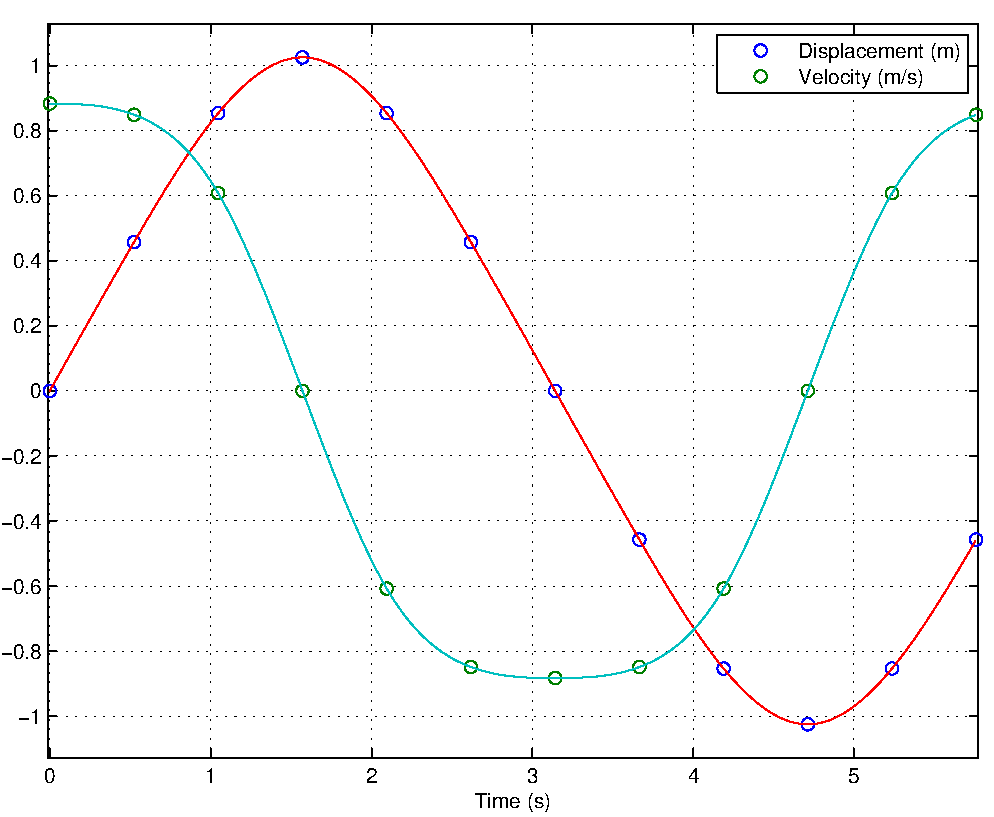
\includegraphics[width=.45\textwidth]{pix/example}}
   \subfigure[Second sub-figure]{
   \label{fig:example_b}
   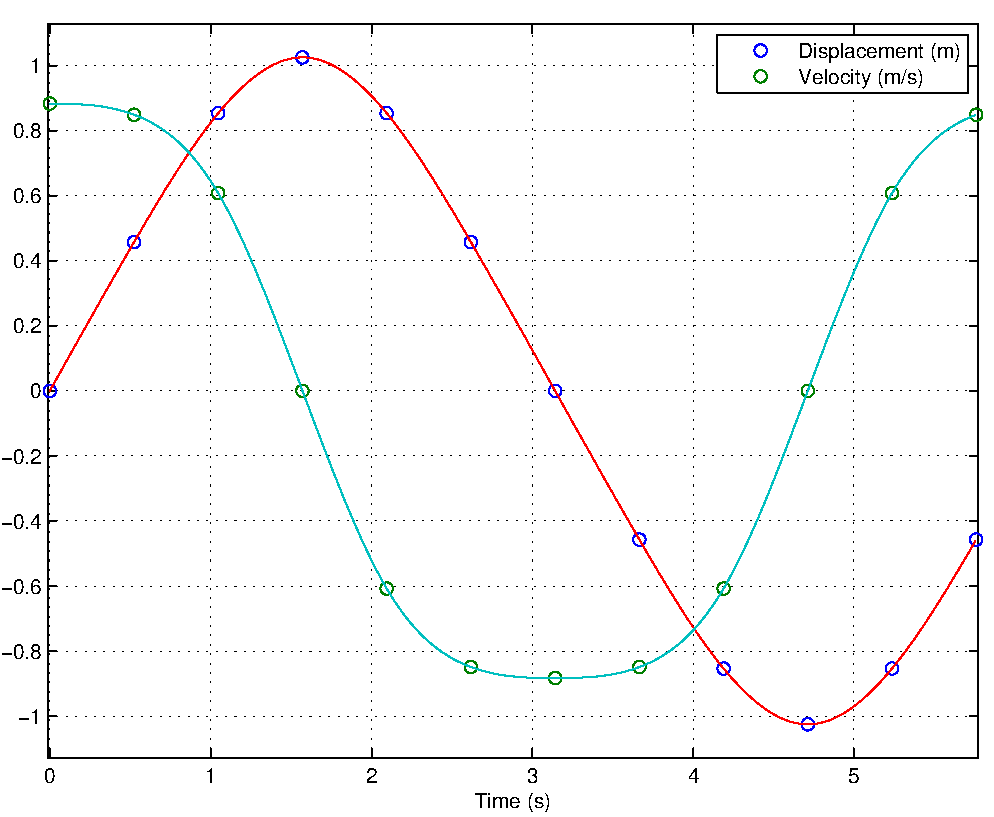
\includegraphics[width=.45\textwidth]{pix/example}}
   \caption{Side-by-side sub-figures.}
   \label{fig:1x2_subfigs}
\end{figure}
%-----------------------------------------------------------------


If you want 4 total figures, just add a line break, \verb'\\', after the second sub-figure as shown in Figure \ref{fig:2x2_subfigs}.  You can add spacing between them with the \verb'\quad' or \verb'\qquad' commands.  There is more space between Figures \ref{fig:example_2x2a} and \ref{fig:example_2x2b} to show the use of this spacing.  Make sure all of your spacing is equal.  And don\rq{}t make your figures this small.  As my advisor told me, \lq\lq{}old people read these\rq\rq{} \cite{Mark}.

%-----------------------------------------------------------------
\begin{figure}[!t]
   \centering
   \subfigure[First sub-figure]{
   \label{fig:example_2x2a}
   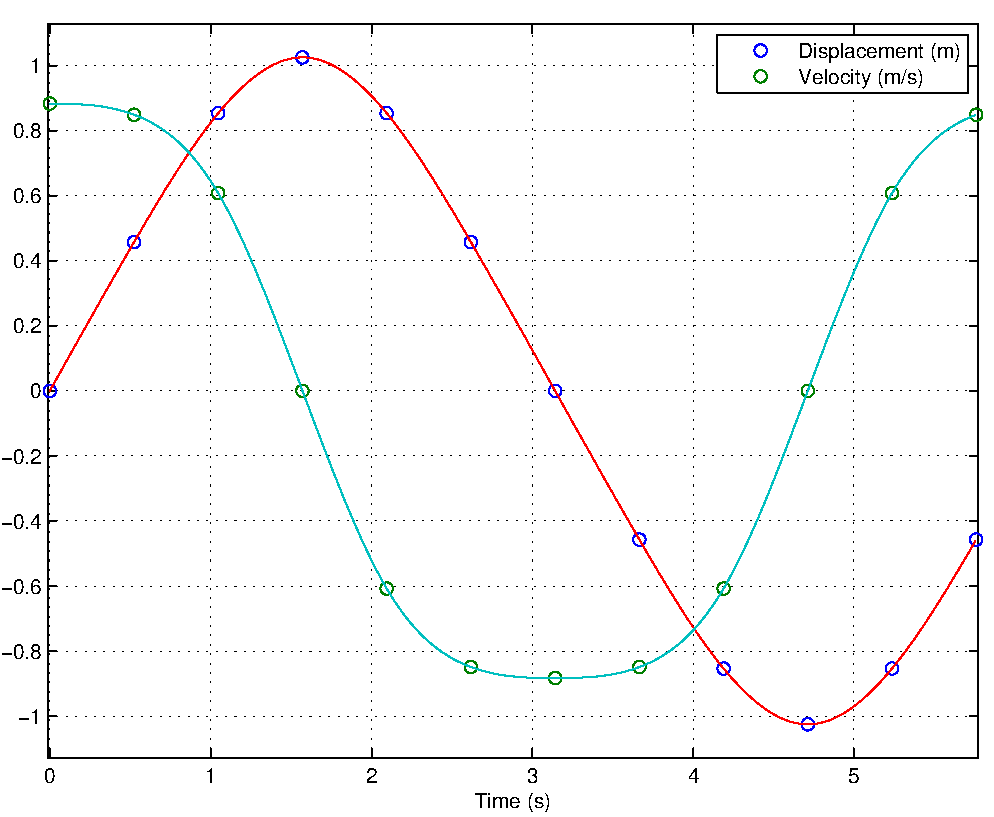
\includegraphics[width=.15\textwidth]{pix/example}} \quad
   \subfigure[Second sub-figure]{
   \label{fig:example_2x2b}
   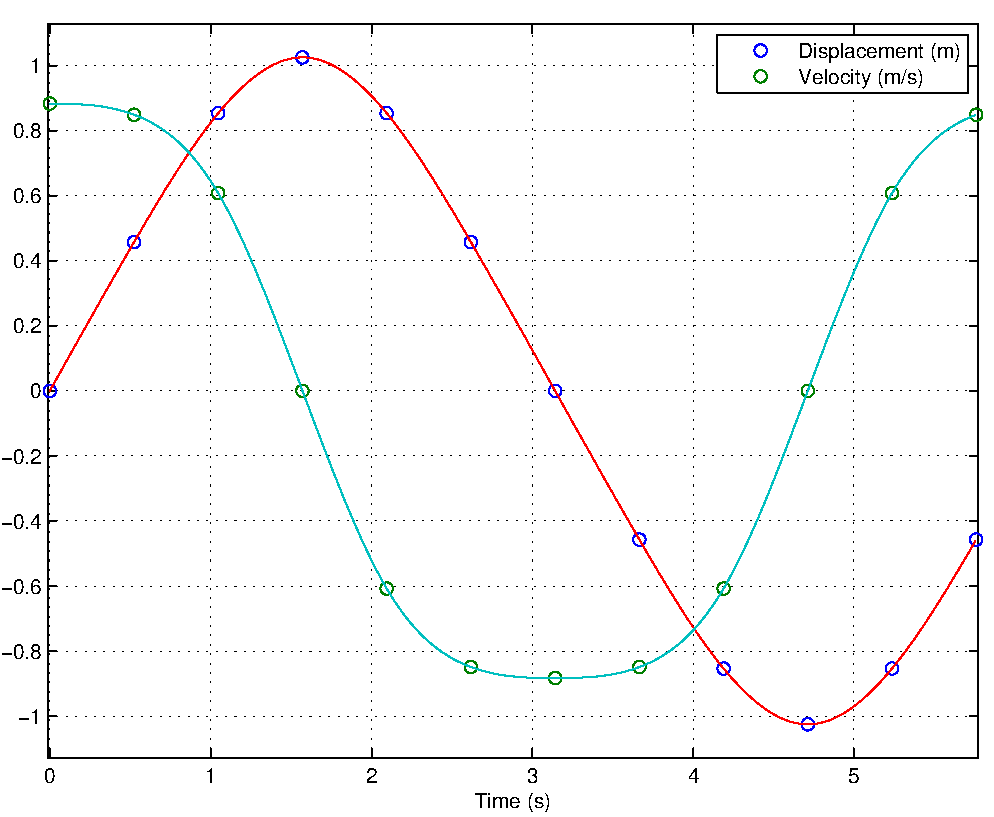
\includegraphics[width=.15\textwidth]{pix/example}}\\
      \subfigure[Third sub-figure]{
   \label{fig:example_2x2c}
   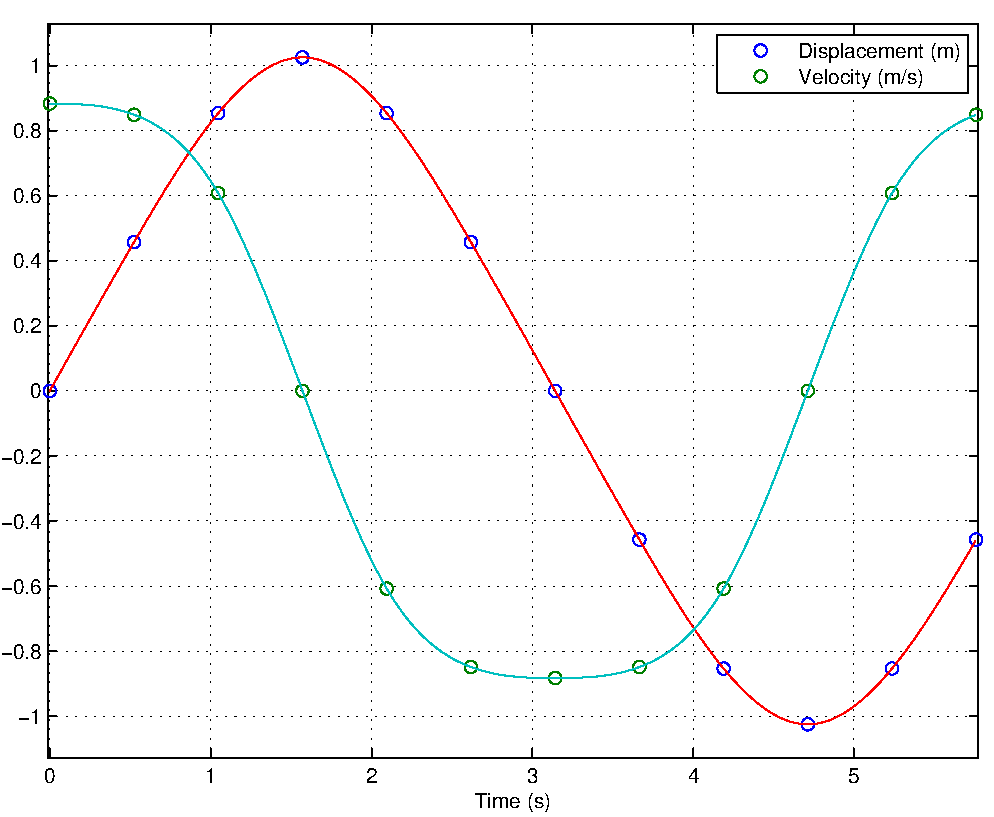
\includegraphics[width=.15\textwidth]{pix/example}}
   \subfigure[Fourth sub-figure]{
   \label{fig:example_2x2d}
   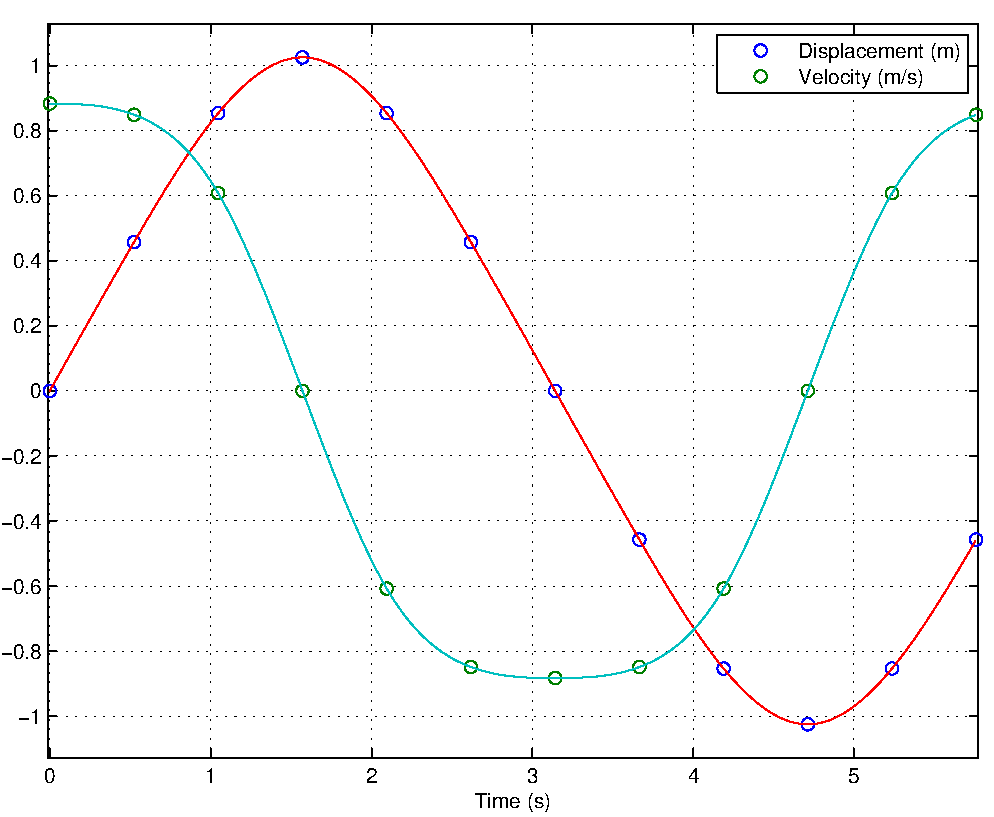
\includegraphics[width=.15\textwidth]{pix/example}}
   \caption{2x2 sub-figures.}
   \label{fig:2x2_subfigs}
\end{figure}
%-----------------------------------------------------------------

%=============================
\section{Including Chapters or Files}
%=============================
You can include chapters using the \verb'\include' command. See the \LaTeX\ file.  Each file can be included separately as to keep editing localized to each chapter.
% ------------------------------------------------------------------------
%\include{chapter2}
% ------------------------------------------------------------------------
%\include{chapter3}
% ------------------------------------------------------------------------

You can also use the \verb'\input' command to include items without forcing a page break.  This becomes handy when generating a table, you can leave the reference in the main document and the table can be updated separately.
\begin{table}[ht] % h - here, t - top, b - bottom, p - page (use a ! to force the table for figure where you want)
  \centering
  \scriptsize % set font size to scriptsize so that table fits within page margins
  \caption{Complete test matrix of waveforms for experimental bench test}
    \begin{tabular}{cccccc}
    \toprule % top line of table
    \textbf{Bandwidth} & \textbf{FFT lines} & \textbf{Samples/Cycle Chirp} & \textbf{Frequency Resolution} & \textbf{Sweep Rate} & \textbf{Sweep Time} \\
	(Hz) 	& 		&	 		& (mHz) & (mHz/sec)	& (sec) \\ \midrule
\multirow{4}[8]{.5in}{\centering8}
		& 100		& 3-10, 20 		& 80    	& 0.64		& 12.5 \\ \cmidrule (l){2-6} % midrule between columns 2-6
		& 200		& 3-10 	     		& 40    	& 0.32 		& 25 \\ \cmidrule (l){2-6}
		& 400   	& 3-10  		& 20   	& 0.16  	& 50 \\ \midrule
%
\multirow{5}[8]{.5in}{\centering16}
		& 100   	& 3-10, 20, 50      	& 160   & 2.56  	& 6.25 \\ \cmidrule (l){2-6}
		& 200   	& 3-10, 20		& 80    	& 1.28  	& 12.5 \\ \cmidrule (l){2-6}
		& 400   	& 3-10, 20     		& 40    	& 0.64  	& 25 \\ \cmidrule (l){2-6}
		& 800		& 3-10      		 & 20    & 0.32  	& 50 \\ \midrule
%
\multirow{6}[12]{.5in}{\centering32}
		& 100   	& 3-10, 20     		 & 320	& 10.24 	& 3.125 \\ \cmidrule (l){2-6}
		& 200   	& 3-10, 20      		& 160	& 5.12  	& 6.25 \\ \cmidrule (l){2-6}
		& 400   	& 3-10, 20      		& 80	& 2.56  	& 12.5 \\ \cmidrule (l){2-6}
		& 800   	& 3-10, 20      		& 40	& 1.28 	 	& 25 \\ \cmidrule (l){2-6}
		& 1600  	& 3-10       		& 20	& 0.64  	& 50 \\ \bottomrule % bottom line of table
    \end{tabular}
  \label{tab:bench_test_matrix}
  \normalsize % reset font size to normal
\end{table}


Using the \verb'booktabs' package makes very professional looking tables by varying the thickness of the lines which can be customized.

%=============================
\clearpage \section{Inserting Code}
%=============================
If you want to insert code you can use the \verb'mcode' package.  You can choose to between several options to frame, have numbered lines , automatic line breaks and more.  Below is an example of listing a MATLAB\textsuperscript{\textregistered} m-file.

\lstinputlisting{importfile.m}

%=============================
\chapter[Programs]{Typesetting Programs using \LaTeX\ }
%=============================
\section{Windows}
%=============================
Below are some programs for Windows:
\begin{itemize}
\item \href{http://miktex.org/}{MiK\TeX}
\subitem- Up-to-date implementation of \TeX 
\subitem- Side-by-side comparison of source and PDF
\subitem- Has portable version that can be run from portable storage device
\item \href{http://www.lyx.org/}{LyX}
\subitem- Graphical interface used with \TeX and \LaTeX\ 
\item \href{http://www.tug.org/texlive/}{\TeX Live} (also Unix)
\item pro\TeX t
\end{itemize}

%=============================
\section{Mac OS}
%=============================
Below are some programs for Mac OS:
\begin{itemize}
\item \href{http://www.lyx.org/}{LyX}
\item\href{http://www.tug.org/mactex/}{Mac\TeX}
\subitem- \TeX Live with the addition of Mac specific programs
\item gw\TeX  (Mac OS X)
\item Latexian (Mac OS X)
\end{itemize}

\section{References}
\label{sec:refs}
\begin{itemize}
\item \href{http://www.ctan.org}{CTAN} home page
\item \href{http://en.wikibooks.org/wiki/LaTeX/}{Wikibooks} \LaTeX\ home page
\end{itemize}


%
%
%-----------------------------------------------------------------------
% Bibliography
%-----------------------------------------------------------------------
\clearpage \phantomsection %used to correctly anchor hyperlinks
\renewcommand\baselinestretch{1.5}
\addcontentsline{toc}{chapter}{Bibliography}
\bibliographystyle{plain}
\bibliography{thesisBIB}
%
%-----------------------------------------------------------------------
% Appendices
%-----------------------------------------------------------------------
%%%%%%%%%%%%%%%%%%%
\begin{appendices}
\phantomsection %use \phantomsection command to correctly anchor hyperlinks
\chapter[An Example Appendix]{Appendix A\\An Example}
\label{chap:AppA}
Here is an appendix\ldots not too difficult.
\phantomsection
\chapter[Another Example Appendix]{Appendix B\\Another Example}
\label{chap:AppB}
Again\ldots not too difficult.
\end{appendices}
%%%%%%%%%%%%%%%%%%%
%
%
%
% End of document
\end{document} 
